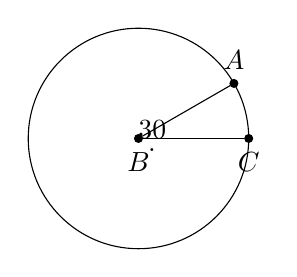
\begin{tikzpicture}
[scale =0.1,>=stealth,point/.style = {draw, circle, fill = black, inner sep = 1pt},]
\node (B) at (0,0)[point,label=below :$B$] {};
\node (C) at (14,0)[point,label=below :$C$] {};
\node (A) at (12.12,6.99)[point,label=above :$A$] {};
\draw (0,0) node [below right] {.} circle (14);
\draw (B)--(A);
\draw (B)--(C);
\tkzMarkAngle[fill=green!40,size=0.1cm,mark=](C,B,A)
\tkzLabelAngle[pos=0.1](C,B,A){\rotatebox{-360}{$30$}}
\end{tikzpicture}

